% Diagram: Metrics Visualization
\begin{figure}[htbp]
\centering
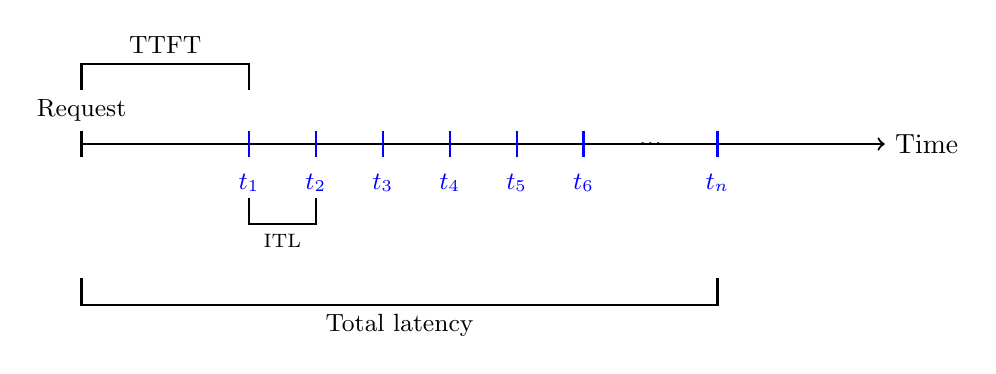
\begin{tikzpicture}[scale=0.85]
% Timeline
\draw[thick, ->] (0, 0) -- (12, 0) node[right] {Time};

% Request marker
\draw[thick] (0, -0.2) -- (0, 0.2);
\node[above] at (0, 0.2) {\small Request};

% TTFT bracket
\draw[thick] (0, 0.8) -- (0, 1.2) -- (2.5, 1.2) -- (2.5, 0.8);
\node[above] at (1.25, 1.2) {\small TTFT};

% First token
\draw[thick, blue] (2.5, -0.2) -- (2.5, 0.2);
\node[below, blue] at (2.5, -0.3) {\small $t_1$};

% ITL brackets
\draw[thick] (2.5, -0.8) -- (2.5, -1.2) -- (3.5, -1.2) -- (3.5, -0.8);
\node[below] at (3, -1.2) {\scriptsize ITL};

% Subsequent tokens
\foreach \x/\n in {3.5/2, 4.5/3, 5.5/4, 6.5/5, 7.5/6} {
    \draw[thick, blue] (\x, -0.2) -- (\x, 0.2);
    \node[below, blue] at (\x, -0.3) {\small $t_{\n}$};
}

\node at (8.5, 0) {...};

% Final token
\draw[thick, blue] (9.5, -0.2) -- (9.5, 0.2);
\node[below, blue] at (9.5, -0.3) {\small $t_n$};

% Total time bracket
\draw[thick] (0, -2) -- (0, -2.4) -- (9.5, -2.4) -- (9.5, -2);
\node[below] at (4.75, -2.4) {\small Total latency};

\end{tikzpicture}
\caption{Inference timing: TTFT is time to first token, ITL is time between subsequent tokens.}
\label{fig:inference-timing}
\end{figure}
